% =====================================================================
%  A1 BETTER POSTER  —  Mike-Morrison-style three-column layout
%
%  Structure (left→right):
%    Left  (~22%, light cream):  project title, authors, sections,
%                                small detailed text (the paper-style
%                                content for people who want depth).
%    Center (~56%, sea image):   ONE big takeaway sentence in massive
%                                type (the "ammo round" — what every
%                                visitor reads in 3 seconds).
%    Right (~22%, light cream):  figure(s), QR code, contact.
%
%  Compile with XeLaTeX (needs Open Sans + Montserrat ExtraBold/Black):
%      latexmk better-poster.tex
% =====================================================================

\documentclass{article}

% Landscape A1 — wider stage for the centre takeaway, common at
% industry / conference poster sessions.
\usepackage[paperwidth=841mm, paperheight=594mm,
            margin=0pt, noheadfoot]{geometry}
\usepackage{fontspec}
\usepackage{xcolor}
\usepackage{graphicx}
\usepackage{tikz}
\usepackage[absolute, overlay]{textpos}
\usepackage{ragged2e}
\usepackage{microtype}
\usepackage[hidelinks]{hyperref}
\usepackage{qrcode}

% Fonts
\setmainfont{Open Sans}
\newfontfamily\headingfont{Montserrat}
\newfontfamily\titlefont{Montserrat ExtraBold}
\newfontfamily\bigfont{Montserrat Black}

% Colour palette
\definecolor{paneltext}{HTML}{1B1B1B}
\definecolor{panelbg}{HTML}{F2EFE8}     % warm cream for side panels
\definecolor{panelmuted}{HTML}{6E6E6E}  % muted body grey
\definecolor{centertext}{HTML}{FFFFFF}
\definecolor{accent}{HTML}{F2C94C}      % yellow highlight for key words

% TextPos in mm
\setlength{\TPHorizModule}{1mm}
\setlength{\TPVertModule}{1mm}
\textblockorigin{0mm}{0mm}

\graphicspath{{../assets/}{assets/}{./}}

\pagestyle{empty}
\setlength{\parindent}{0pt}
\setlength{\parskip}{0.55\baselineskip}
\linespread{1.18}

% Column geometry (mm). Landscape A1: 22/56/22 split of 841 mm width.
\newcommand{\leftColW}{185}    % left column width
\newcommand{\centerColX}{185}  % x where center column starts
\newcommand{\centerColW}{471}  % center column width
\newcommand{\rightColX}{656}   % x where right column starts
\newcommand{\rightColW}{185}   % right column width
\newcommand{\panelPad}{14}     % inner padding (mm) inside side panels

% Side-panel section heading
\newcommand{\panelhead}[1]{%
  \par\addvspace{6mm}%
  {\headingfont\bfseries\fontsize{15pt}{18pt}\selectfont
   \MakeUppercase{#1}\par}%
  \nopagebreak\vspace{1mm}%
  \textcolor{accent}{\rule{32mm}{1.5pt}}\par
  \vspace{2mm}%
}

% Helper to highlight a phrase inside the big takeaway
\newcommand{\hl}[1]{\textcolor{accent}{#1}}

\begin{document}

% ---------------------------------------------------------------------
%  BACKGROUND PANELS
% ---------------------------------------------------------------------
\begin{tikzpicture}[remember picture, overlay]
  % Left & right cream panels
  \fill[panelbg]
     (current page.north west)
     rectangle
     ([xshift=\leftColW mm]current page.south west);
  \fill[panelbg]
     ([xshift=\rightColX mm]current page.north west)
     rectangle
     (current page.south east);
  % Center band: sea_grad.png cropped to fit the centre column.
  % Image is 2250×4000 px; column aspect = 471/594 ≈ 0.793 →
  % keep a 2250×2837 strip at the bottom of the image so the dark
  % gradient lands at the bottom of the column.
  \node[anchor=north west, inner sep=0pt]
     at ([xshift=\centerColX mm]current page.north west)
     {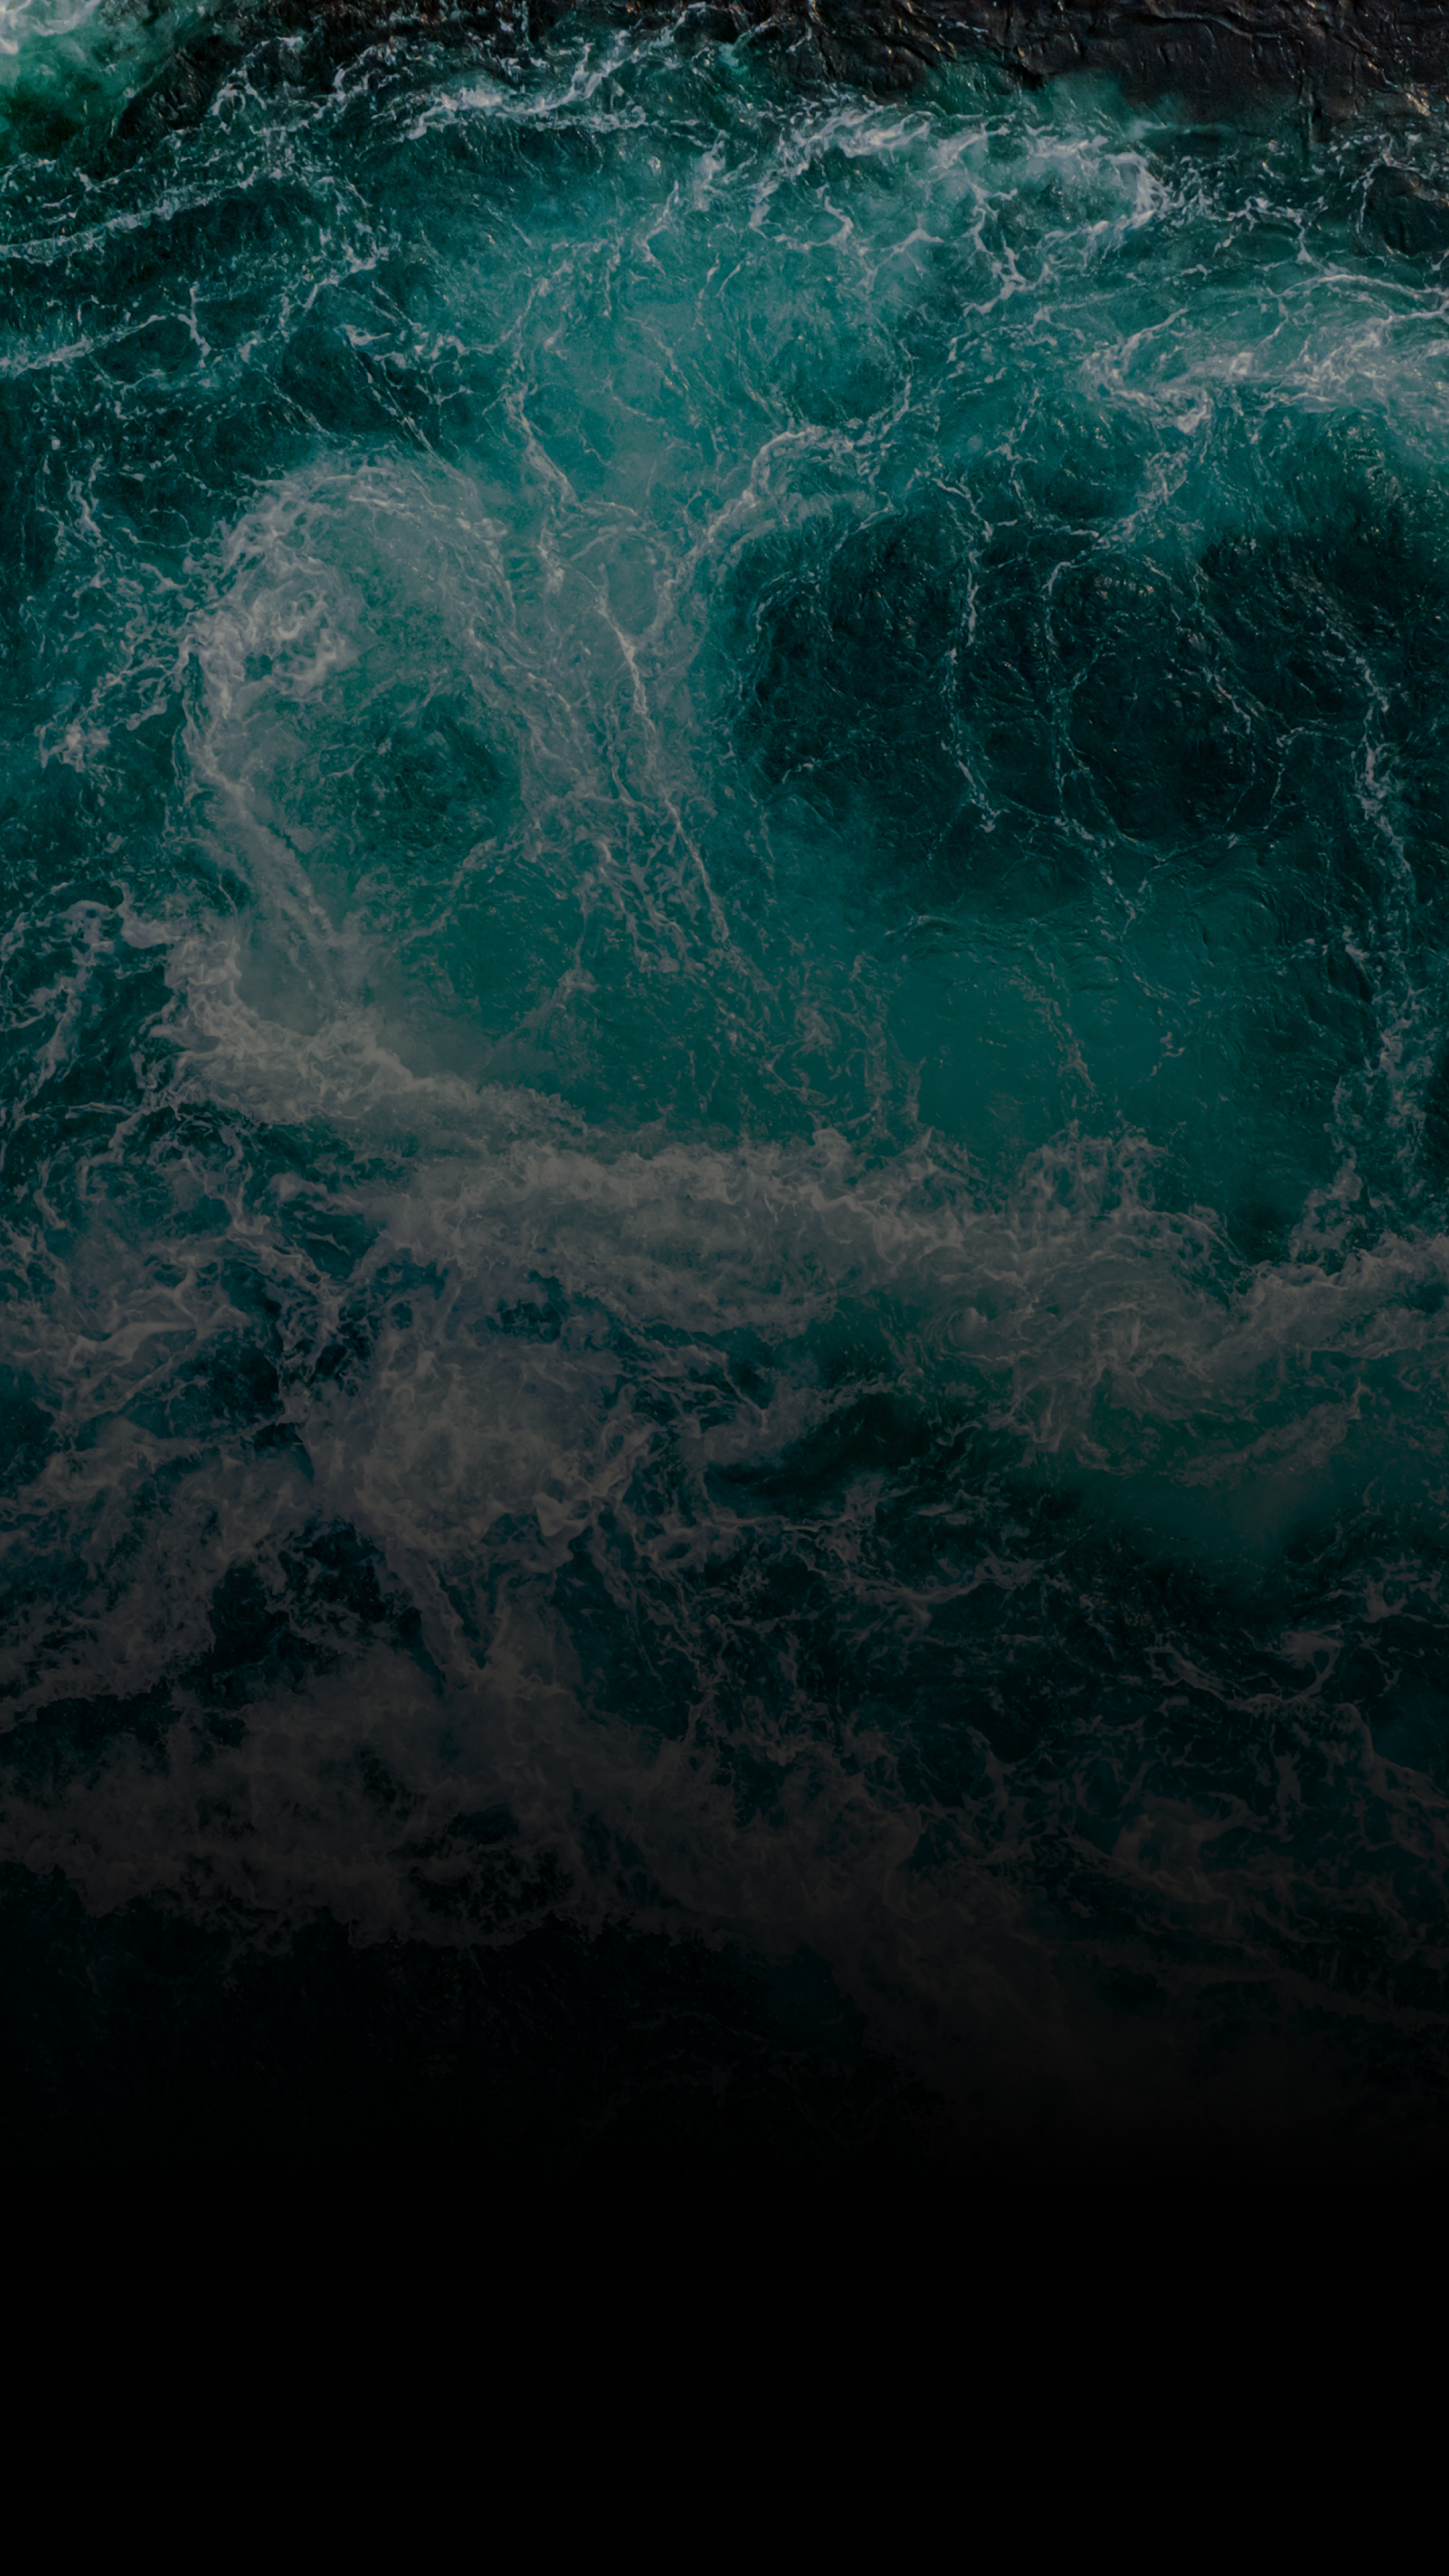
\includegraphics[width=\centerColW mm,
                       viewport=0 0 2250 2837, clip]{sea_grad.png}};
\end{tikzpicture}

% ---------------------------------------------------------------------
%  LEFT COLUMN — paper-style content
% ---------------------------------------------------------------------
\begin{textblock}{157}(14,18)                   % 185 - 2*14 = 157 mm wide
  \color{paneltext}\fontsize{12pt}{16pt}\selectfont\RaggedRight

  % Project title (small at top)
  {\headingfont\bfseries\fontsize{20pt}{24pt}\selectfont
   Untapping the Hidden Potential of Non-Textual Maritime Data Using AI\par}
  \vspace{6mm}

  {\fontsize{10pt}{13pt}\selectfont
   \textbf{Lamin Jatta}\\
   Maritime Technology, Novia UAS\\
   first.last@novia.fi\par
   \vspace{2mm}
   \textbf{Supervisors:} Andreas Lundell (ÅAU),
   Johan Westö (Novia UAS), Mikael Manngård (Novia UAS).\par}

  \panelhead{Background}
  Industries like maritime and automotive generate massive amounts of
  audio and video data, only a small fraction of which is relevant for
  training AI. Engineering data is rarely available in machine-readable
  form — it's locked in figures, drawings, and diagrams.

  \panelhead{Approach}
  AI methods — natural language processing, multimodal embeddings, and
  semantic search — are applied to extract, organise, and retrieve
  relevant information from non-textual data and represent it in a
  structured form.

  \panelhead{Outcomes}
  Four planned papers:
  \begin{itemize}\setlength{\itemsep}{1pt}\setlength{\parsep}{1pt}
    \item[I.] Maritime Automatic Speech Recognition and Key-Phrase Extraction.
    \item[II.] Semantic Search for Maritime Unstructured Data.
    \item[III.] Graph Representations of Maritime Systems.
    \item[IV.] Information Extraction from Engineering Graphs and Diagrams.
  \end{itemize}

  \panelhead{Timeline}
  Conducted in the Virtual Sea Trial project,\\
  1 Jan 2024 -- 31 Dec 2026.

  \vfill
  {\color{panelmuted}\fontsize{9pt}{12pt}\selectfont
   Novia University of Applied Sciences \\ Åbo Akademi University\par}
\end{textblock}

% ---------------------------------------------------------------------
%  CENTER COLUMN — logos top, big takeaway middle, footer bottom
% ---------------------------------------------------------------------
% Logos at top of center column
\begin{textblock}{443}(199,28)                  % centerColX (185) + 14 padding
  \color{centertext}
  \begin{minipage}[c]{\linewidth}
    
\includegraphics[height=38mm]{abo_akademi_university-logo_white.png}\hfill
    
\includegraphics[height=22mm]{logoinvinternwhite.pdf}
  \end{minipage}
\end{textblock}

% BIG TAKEAWAY — vertically centred area
\begin{textblock}{443}(199,160)
  \color{centertext}\centering
  {\bigfont\fontsize{96pt}{110pt}\selectfont
   Make every minute of maritime
   \hl{audio, video, and 3D}
   searchable like text.\par}
  \vspace{18mm}
  {\headingfont\fontsize{28pt}{36pt}\selectfont
   So engineers can test ships
   \emph{virtually} instead of at sea.\par}
\end{textblock}

% Funding line at bottom of center column
\begin{textblock}{443}(199,560)
  \color{centertext}\centering
  \fontsize{12pt}{15pt}\selectfont
  Funded by Business Finland · Co-Innovation Project Virtual Sea Trial · virtualseatrial.fi
\end{textblock}

% ---------------------------------------------------------------------
%  RIGHT COLUMN — figure + QR + contact
% ---------------------------------------------------------------------
\begin{textblock}{157}(670,18)            % rightColX (656) + panelPad (14)
  \color{paneltext}\fontsize{12pt}{16pt}\selectfont\RaggedRight

  \panelhead{Key Idea}
  Voice + video + 3-D models are first-class data, not byproducts.
  Treat them like text and a whole search index opens up.

  \panelhead{What Industry Gets}
  \begin{itemize}\setlength{\itemsep}{2pt}\setlength{\parsep}{1pt}
    \item Less time scrubbing through hours of sea-trial footage.
    \item Automated tests built from real captured behaviour.
    \item Engineering drawings that answer questions, not just sit in PDFs.
  \end{itemize}

  \panelhead{Read More}
  \vspace{2mm}
  \begin{center}
    \qrcode[height=44mm]{https://virtualseatrial.fi}
  \end{center}
  \vspace{1mm}
  \centering virtualseatrial.fi

  \vfill
  {\color{panelmuted}\fontsize{9pt}{12pt}\selectfont
   Industry presentation\\Vaasa, 2026\par}
\end{textblock}

\end{document}
